\section{User Interface}

The user interface (UI) for Stegosaurus is going to be created in Visual Studio using C\# and Windows Forms.
In some of our previous experiments, we have created a very basic UI.
The only function these UIs could was to show the cover image, the hidden image and then the output.
In this example, the user had no visual cue on whether the programme had done as it was supposed to.
This is something that we would like to improve on in our final design.

Something else the experiment lacked was a choice of encoding.
For example, whether they would like to use the least significant bit method or our graph theoretical method.
Therefore, the final design should also include several different options, so as to customise the encoding of their image to something that suits their requirements.

Another thing lacking in previous designs has been a guide through the programme and its functions together with a description of what they do.
Previous versions have been less complex and perhaps did not require much explanation.However, now as the programme will have a larger set of different settings, we believe that it should be a requirement to have a short explanation of these, what impact they will have on the end result and what the programme will do in general.

All of these things should illustrate to the user how the programme works and what it is doing when running.

\subsection{Design}

The figure as shown in \ref{fig:LSBForm} is what our UI looked like for our LSB experiment.
We are taking the main ideas from this, where we show the user the images they have selected and the final product.
\begin{figure}
	\centering
	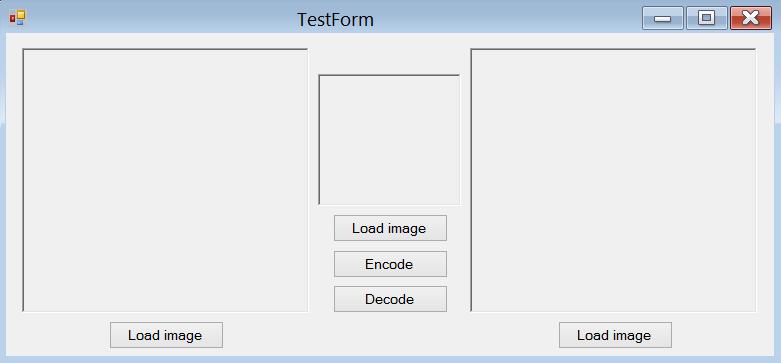
\includegraphics[width=1\textwidth]{figures/LSBForm.png}
	\caption{LSB Form.}
	\label{fig:LSBForm}
\end{figure}
We decided, however, that it was confusing to have three load buttons.
As in the figure described before, the clean image is uploaded on one side, the message in the middle and the encoded image on the right.
And when you wanted to decode the image, the encoded image had to be uploaded on the right.
Because of this we have therefore decided to only have two buttons, one for loading an image that is to be encoded or decoded and another for only loading the hidden message.

We have decided to include some extra features to our overall design.
These features include giving the user options to use their own huffman code and own quantization tables to make their encoded image as precise as possible.

To do this, we decided that creating an options form would be best when it comes to guiding the user through our programme.
The options box would consist of quality settings, choice of encoding method, customisation of Huffman tables and customisation of quantization.
However, there are also default options, if the user in question has no specific preferences.

All of these options allow the user to encode their image according to their specific needs.
After the image has been encoded, there is, naturally, a need to be able to decode the image.
This means that the programme should be able to present these options to the user as openly as possible, as these are the key features of the programme.

This, however, is slightly more advanced when it came to huffman coding as each channel has a different size.

As something more general, we have created a basic help guide to explain to the user how the programme works, and a short description of what each feature entails.
Within this section, there will also be an 'about' that gives a description of what the programme is for and who it is by.

Something that is absolutely fundamental to the programme, is showing the user the images they provide and the image they produce.
This visual representation gives the user an indication that the programme is doing something and also peace of mind in that they have chosen the correct files.

Another thing in regards to giving the user a visual representation is having some form of status indicator, to show the user that the programme is working on encoding or decoding their image.

Likewise, another feature, that we deem to be a rather important visual representation is the quality level of encoding.
Therefore, we have decided to have a slider to show what level of quality the programme will produce.

The following list is what the user interface will include:

\begin{description}
\item[Main form]
The encode and decode buttons work as they are.
But if we also want to have our buttons to work as an option on whether the image has to be encoded or decoded, radio buttons, where encode or decode get selected, and thereby when decode is selected then the message image load button, will not be applicable for selection.

In our original design, we had a maximize and minimise button next to close.
We have since decided on changing this, so that the maximise and minimise buttons are disabled.
This is to stop any change of size in the programme, so that all features of the programme retain their original size.
This is shown in our main form as can be seen on figures \ref{fig:StegoLSBMain} and \ref{fig:StegoGTAMain}.

\item[LSB or Graph Theory Method]
The user will be able to switch between methods by clicking on a tab that will be shown at the top of the main form.
This idea seems more effective than our initial idea of having the option of selecting which method in an options form.
Having the option to toggle between the two on the main form makes it much clearer what this programme can do.

\begin{figure}
	\centering
	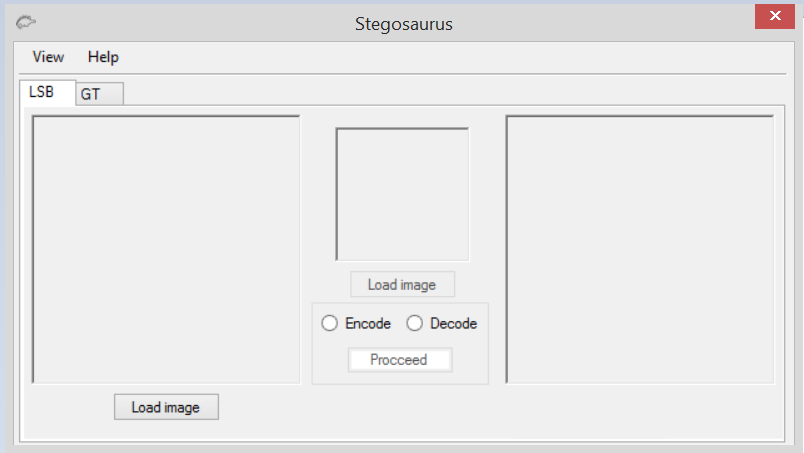
\includegraphics[width=1\textwidth]{figures/StegoLSBMain.png}
	\caption{This is almost identical to previous experiment, although with some changes as mentioned previously.}
	\label{fig:StegoLSBMain}
\end{figure}

\begin{figure}
	\centering
	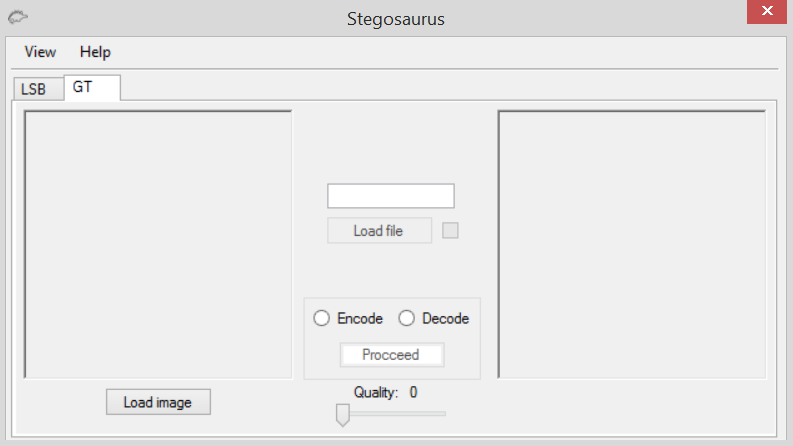
\includegraphics[width=1\textwidth]{figures/StegoGTAMain.png}
	\caption{This is how the user will meet our graph theoretical method, where there is no longer an option for inserting an image to be encoded.}
	\label{fig:StegoGTAMain}
\end{figure}

\item[Quantization Tables]
A difficulty that arose when deciding on these features were: how we were going to make it possible for a user to input their custom quantization and huffman codes.
An initial idea included a CSV-file (Comma Separated Values file), but we decided that for quantization tables, it was ideal and no trouble to have the user input their table by typing it in text boxes as the size of each quantization table is the same for both the luminance and chromium channels.
This can be seen in \ref{fig:StegoOptionQuant}.

\begin{figure}
	\centering
	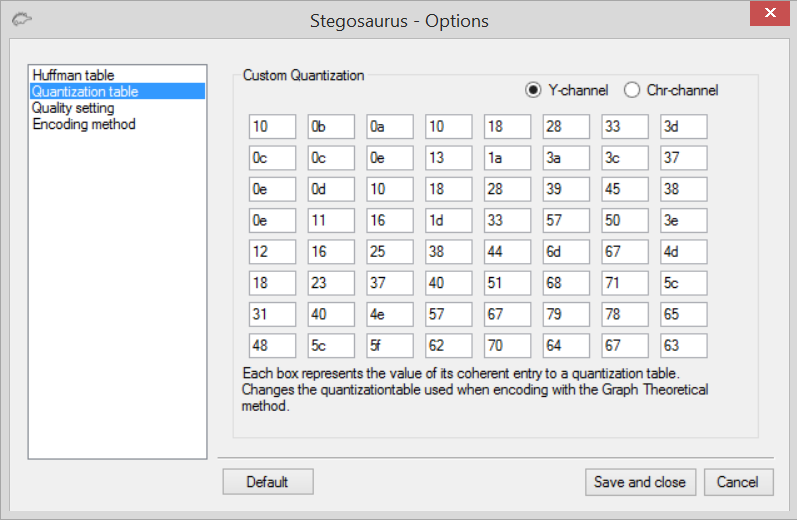
\includegraphics[width=1\textwidth]{figures/StegoOptionQuant.png}
	\caption{This is how the custom quantization table is shown to the user.}
	\label{fig:StegoOptionQuant}
\end{figure}

\item[Huffman Tables]
Huffman tables requires a similar form to quantization tables.
There are four radio buttons to switch between the four different channels.
Text boxes have been set up to be able to take in a string from the user.
However, as the sizes of the huffman tables vary, it is necessary to have a function that allows the user to add rows as needed.

\begin{figure}
	\centering
	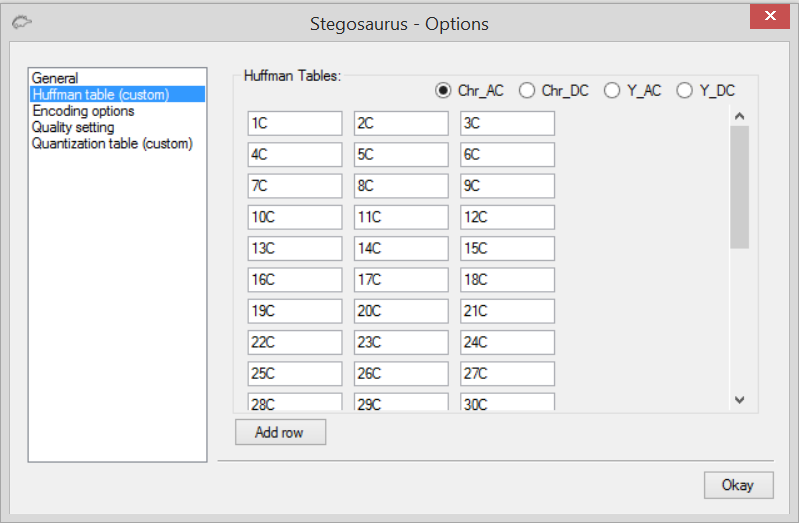
\includegraphics[width=1\textwidth]{figures/StegoOptionHuff.png}
	\caption{The picture above shows how the user will see the Huffman table.}
	\label{fig:StegoOptionHuff}
\end{figure}

\item[Quality setting]
Our initial idea was a slider that would be shown on the main form and in our options form.
This slider would then tell us what the quality settings were set to, from 0 to 100.
This slider was initially planned to be a part of the main form, but has since been moved to options setting and the main form for the graph theoretical, as we decided it was as much a custom option as the Huffman and quantization tables.

\item[Progress bar]
The original idea of showing the user what was happening with the programme by having a pop-up window has been replaced by having a loading sign by the cursor.
This is also a way of showing the viewer that something is happening.
If the implementation took more than a few minutes, it would maybe be more of a requirement, but as the programme works rather quickly, it does not seem necessary.

\item[Help form]
A very general description of what the programme does and descriptions of the different settings in the options form.
We believe this to be important to the overall understanding of how the programme is to be used; something that our previous experiments have not had.
\end{description}

\subsection{Possible Improvements}
There are some things with the UI that can be seen as problematic.
As the programme is now, there is no option to save one's custom settings when the programme is closed.
This could have been a useful tool, as some of the components are quite time consuming, especially writing each value in the Huffman Tables and quantization table forms.

This in of itself is also an issue.
Typing each value in the different text boxes can be quite cumbersome and not having a way of saving one's work, makes the idea of having the option for custom features almost redundant.
However, for quick custom features, such as quality settings, the fact that it is not saved when the programme is closed, is not such a problem.

These reasons made it clear to us, that it should be mandatory for us to make it possible for the user to save their details, so the long process of typing in each value, was not a necessity each time the programme was opened.

This new interface has advantages over previous interfaces in our experiments throughout our process, but there are still some features that could be included, not to improve the programme, but the overall user experience.


